%% Quick summary of HSE models.rnw

\documentclass{article}\usepackage{graphicx, color}
%% maxwidth is the original width if it is less than linewidth
%% otherwise use linewidth (to make sure the graphics do not exceed the margin)
\makeatletter
\def\maxwidth{ %
  \ifdim\Gin@nat@width>\linewidth
    \linewidth
  \else
    \Gin@nat@width
  \fi
}
\makeatother

\IfFileExists{upquote.sty}{\usepackage{upquote}}{}
\definecolor{fgcolor}{rgb}{0.2, 0.2, 0.2}
\newcommand{\hlnumber}[1]{\textcolor[rgb]{0,0,0}{#1}}%
\newcommand{\hlfunctioncall}[1]{\textcolor[rgb]{0.501960784313725,0,0.329411764705882}{\textbf{#1}}}%
\newcommand{\hlstring}[1]{\textcolor[rgb]{0.6,0.6,1}{#1}}%
\newcommand{\hlkeyword}[1]{\textcolor[rgb]{0,0,0}{\textbf{#1}}}%
\newcommand{\hlargument}[1]{\textcolor[rgb]{0.690196078431373,0.250980392156863,0.0196078431372549}{#1}}%
\newcommand{\hlcomment}[1]{\textcolor[rgb]{0.180392156862745,0.6,0.341176470588235}{#1}}%
\newcommand{\hlroxygencomment}[1]{\textcolor[rgb]{0.43921568627451,0.47843137254902,0.701960784313725}{#1}}%
\newcommand{\hlformalargs}[1]{\textcolor[rgb]{0.690196078431373,0.250980392156863,0.0196078431372549}{#1}}%
\newcommand{\hleqformalargs}[1]{\textcolor[rgb]{0.690196078431373,0.250980392156863,0.0196078431372549}{#1}}%
\newcommand{\hlassignement}[1]{\textcolor[rgb]{0,0,0}{\textbf{#1}}}%
\newcommand{\hlpackage}[1]{\textcolor[rgb]{0.588235294117647,0.709803921568627,0.145098039215686}{#1}}%
\newcommand{\hlslot}[1]{\textit{#1}}%
\newcommand{\hlsymbol}[1]{\textcolor[rgb]{0,0,0}{#1}}%
\newcommand{\hlprompt}[1]{\textcolor[rgb]{0.2,0.2,0.2}{#1}}%

\usepackage{framed}
\makeatletter
\newenvironment{kframe}{%
 \def\at@end@of@kframe{}%
 \ifinner\ifhmode%
  \def\at@end@of@kframe{\end{minipage}}%
  \begin{minipage}{\columnwidth}%
 \fi\fi%
 \def\FrameCommand##1{\hskip\@totalleftmargin \hskip-\fboxsep
 \colorbox{shadecolor}{##1}\hskip-\fboxsep
     % There is no \\@totalrightmargin, so:
     \hskip-\linewidth \hskip-\@totalleftmargin \hskip\columnwidth}%
 \MakeFramed {\advance\hsize-\width
   \@totalleftmargin\z@ \linewidth\hsize
   \@setminipage}}%
 {\par\unskip\endMakeFramed%
 \at@end@of@kframe}
\makeatother

\definecolor{shadecolor}{rgb}{.97, .97, .97}
\definecolor{messagecolor}{rgb}{0, 0, 0}
\definecolor{warningcolor}{rgb}{1, 0, 1}
\definecolor{errorcolor}{rgb}{1, 0, 0}
\newenvironment{knitrout}{}{} % an empty environment to be redefined in TeX

\usepackage{alltt}
%\documentclass{scrartcl}   % Koma-script version -- many collisions with the packages below

\usepackage{geometry}
\geometry{verbose,tmargin=2.5cm,bmargin=2.5cm,lmargin=3.5cm,rmargin=3.5cm}
\usepackage[titletoc]{appendix}
\usepackage{pdfpages}
%\usepackage[draft]{pdfpages} % Just inserts a placeholder

\usepackage{graphicx}  % For inserting existing images
\usepackage{float}     % Helps make sure that float placement options like H work

\usepackage{parskip}   % Insert a blank line between paragraphs

\usepackage{booktabs}  % Nice toprules and bottomrules
\heavyrulewidth=1.5pt  % Change the default to heavier lines

\usepackage{placeins}  % Float barriers to keep floats from drifting down

\usepackage[bookmarks]{hyperref} % Make bookmarks in the compiled pdf

\usepackage{comment}   % Allows block comments ... begin{comment} end{comment}
                       % Surrounding knitr chunks -- chunks will execute, but output will not weave into pdf  6/20/13
                       % This is often satisfactory, and speeds up compliation dramatically ... 
                       %    but if a chunk has an error then compilation will halt
                       % Can always use % to comment out chunks
                       % Can also set a "dothis" variable to FALSE in a chunk, then in subsequent chunks set option eval=dothis
                       
% For package xtable
\usepackage{booktabs}  % Nice toprules and bottomrules
\heavyrulewidth=1.5pt  % Change the default to heavier lines
\usepackage{longtable} % Tables that span more than one page
\usepackage{rotating}  % To rotate a page sideways
\usepackage{tabularx}  % To control the width of the table

\usepackage{changepage} % Temporarily change margins -- helpful for wide xtables

% Watermark packages
% \usepackage[firstpage]{draftwatermark}
% \SetWatermarkText{Confidential}
% \SetWatermarkScale{5}
%\SetWatermarkColor[rgb]{0.7,0,0}      % Make text red

%\begin{comment}


%\end{comment}




\begin{document}


\title{ Quick summary of HSE models for forecasting mesothelioma incidence \\ Internal document  }
\author{Timothy Wyant}
\date{ 8/30/13}
\maketitle

\tableofcontents
\listoffigures

\section{Introduction}
As I mentioned in an email, I would like you to undertake a project involving estimating a form (or several forms) of the so-called HSE model of mesothelioma incidence in the U.S.  I would then like you to forecast future annual mesotheliomas in the U.S. using one or more of these models, along with some error bounds.  Finally, we will use these national forecasts to make forecasts for individual asbestos trusts.  Typically, I do this by (1) calculating the ratios of recent mesothelioma claims counts against a trust to national counts, by birth cohohrt, and (2) applying these ratios to future predicted national incidence counts from your model, again by birth cohort.

The HSE model is basically a poisson regression of mesothelioma incidence as a function of past exposure.  The poisson mean for any birth cohort in a given year is somewhat complex nonlinear function of cumulative exposure, and some biomedical parameters related to latency, intensity of exposure, and the manner in which risk increases as a function of time since exposuree.  

This note provides some background on the HSE models, and other models that have been used to forecast asbestos claims. This note also outlines issues that have arisen regarding design and fitting of mesothelioma incidence models, and the treatment and use of demographic, historic incidence, and exposure data that provide the independent varialbes for the fitting.

Along with this note, I am providing a zipped directory that contains: 

\begin{enumerate}
  \item PDFs of relevant references,
  \item A summary xls that provides a master list of all the references by category,
  \item Demographic and mesothelioma incidence data,
  \item Summaries of my previous fits of the HSE and other models,
  \item An Rstudio project that includes the Rnw program that produces this document, along with some R programs that process demographic and incidence data.
\end{enumerate}

For purposes of this note, I have created my own idiosyncratic bibliographic reference system.  The summary xls mentioned above crosswalks the references to the pdf files in the zipped directory.

This background note does not pretend to be an exhaustive discussion of mesothelioma model fitting and forecasting issues, but hopefully it will give you a good start.


\section{Projecting mesothelioma incidence}

Mesothelioma has a long latency, so even though U.S. occupational exposure ended (in theory, and disregarding some more recent exposure for brake mechanics) around 1980-1982, we expect to see mesothelioma claims against these trusts until around 2060.  \footnote{ You'll see 2050 as the furthest year in a lot of projections, including some of mine.  This is because it has been relatively recently that reevaluation of the demographics of exposed workers has suggested that we need to move the outer boundaries further into the future.  In truth, it doesn't matter very much, because there are not many claims projected to occur in the 2050s.  Other uncertainties in the forecasting process are generally an order of magnitude greater than the uncertainty regarding the scale of continued incidence after 2050.  But we should gradually modify our forecasts to go out to 2060.}  Generally, the annual number of mesothelioma claims against one of our trusts is assumed to be a fixed fraction of the U.S. and Canadian mesotheliomas.  Canadian claims are generally treated as U.S. domestic claims, in terms of trust evaluation rules and level of compensation.  (There are many fewer Canadian mesotheliomas than there are U.S. mesotheliomas, or course, just because of the difference in population size.)  Now, "fixed" should be in quotes because sometimes (especially with a small trust) additional exposure worksites are identified for a given defendant.  And when a new trust comes online after a long time in bankruptcy (when new claim filings are stayed by the bankruptcy process) it may be difficult to know exactly what the fixed fraction is.  But caveats aside, we usually assume a fixed fraction.  This fraction in the asbestos expert witness vernacular -- aka "the lingo" in this document -- is often referred to as the "propensity to sue".

Mesothelioma is almost entirely caused by asbestos exposure, and most of that exposure is occupational.  In addition, there are reasonably good models of how risk increases as a function of time since first exposure, and of level of exposure.  This summary note is full of qualifiers like "generally" and "reasonably good" because, as you might imagine, given the disputatious environment in which we find ourselves, almost every element of a set of calculations has been or will be a cause for disagreement.  Nonetheless, the forest is still a lot bigger than the individual trees, so I will try in this note to focus on the former with periodic asides about the latter.   Mesothelioma forecasting is central to:

\begin{enumerate}
  \item Determine how many mesothelioma are likely to be filed in the future against a trust, and when.  (The "when" is important because a trust can earn money on its investments, so timing as well as quantity are elements of the cash flow models.)  We do this by first making a national projection of mesothelioma incidence, and then applying a propensity to sue.  The declining curves of expected future incidence have different monikers in the lingo, such as "future decline curves" or "runoff curves."
  \item Assess "how bad it can get" -- many of the large trusts have mesothelioma filing rates that are close to the national incidence rates.  So the national incidence rates provide an upper bound in worst-case scenarios.  As you've seen, I superimpose a national incidence curve on the bar charts in our quarterly reports.
  \item Because mesothelioma is so closely tied to asbestos exposure, and has a developed science, projections of other diseases and conditions (lung cancer, colorectal and other digestive tract cancers, asbestosis) are often derived as some function of meosthelioma incidence.  This is done by either applying some ratio to meso incidence, or "inverting" meso incidence to calculate the demographic profile of exposed workers likely to file claims against a given trust, and then applying some disease-specific exposure-risk model to this estimated exposed worker population. 
\end{enumerate}


\section{Mesothelioma projection methods}

Okay, so what is the HSE model?  HSE stands for "Health Safety Executive," a UK government agency that is sort of a hybrid of OSHA and the CDC.  Among other things, HSE tracks and report mesothelioma incidence (a lot better than we do).  And they have been active in recent years in creating and using new models for mesothelioma forecasting.  Note that I say "models".  Not only have they fit different models, but every time they fit "the same" model they tinker with it, so there are  models 1a, 1b, 1c, 2, 3, etc.  On top of that, the basic models have been adopted by actuaries and public health folks in the UK and in Australia, and with some of us here in the asbestos trust world.  All of us secondary adopters have done our own tinkering as well.  So "HSE model" is really more of a genus than a species.

Here is a brief (and not exhaustive) overview of projection methods that are, or have been in use:

\begin{enumerate}
  \item \textbf{Nicholson method.}  From William Nicholson, in 1983.  This is a nice piece of work, but arguably dated.  He took airborne asbestos fiber concentration data from several industrial hygiene studies, BLS data on employment by industry, risk as a function of time since exposure from a longitudingal study of insulators, and NHIS death rates, and forecast future mesothelioma and lung cancer incidence. 
  
The most common method that experts have used in asbestos bankruptcy proceedings over the past decadesd has been to calculate a "propensity to sue" for a particular debtor, and apply it to Nicholson forecasts to get projecte claims.  However, the industries that generate the majority of today's claims are not industries that Nicholson included.  In particular, the new industry have much younger workforces.  Nicholson did not model women, or family members of exposed workers.  (It takes very little exposure to elevate the risk of mesothelioma.  Whenever an asbestos worker came home from work and bounced a kid on his or her knee, or handed a spouse some overalls to was, he was creating a poential mesothelioma case.)  Nicholson looked only at U.S. incidence.  He attenuated his worker cohorts in the future by applying death rates that were valid in the 1970s, not today's lower death rates.  His risk-as-a-function-of-exposure models have been modified and updated in the epidemiology literature. 

This method is still used by some experts, most notably by the experts for the TACs -- each trust has a Trust Advisory Committee made of lawyers representing current claims.  These experts have principled reasons for espousing the Nicholson method, but I would be remiss if I did not note in passing that this method yields lower future meso counts -- by as much as 30-35\% -- than all other methods currently in use. 

\item \textbf{KPMG Nicholson} Along about 2000-2005, KPMG did an updated version of the Nicholson method that essentially replicated his work, but updating the industeries (and their workforce age profiles) included in the calculation.

\item \textbf{Revised KPMG Nicholson}  In 2010 or thereabouts, ARPC (a firm that for while was a subsidiary of KPMG, and is now both the claims administrator and the forecasting expert for many trusts), at my urging, updated KPMG Nicholson with current and projected U.S. death rates.

\item \textbf{Peto method} In 1990, ARPC asked me to come up with a metod for forecasting mesothelioma claims for the UNR trust.  The Nicholson method was not widely in use at the time.  I came up with what is called an inversion method -- I took meso claims, calculated the inverse of the risk-as-function-of-time-since-exposure formula, estimated the size and age profile of the exposed workforce for this trust, and moved this workforce forward in time, applying death rates and probabilities of disease in each futue year.  Unbeknownst to me, the Brit epidemiologist Julian Peto had done something similar, so ARPC at some subsequent date rechristined this approach as "the Peto method".  ARPC also refined my original methods for calclating future lung and other cancers, and nonmalignants, as a function of mesoteliomas.

Somewhere in the late 1990s, ARPC also started using a simple model averaging for their forecasts -- they took the median forecast in each future year of the Nicholson, the KPMG Nicholson, and the Peto methods.

\item \textbf{Revised Peto method}  In 2010 or thereabouts, experts for the TAC in the BW Trust challenged the Peto method.  In fact, this challenge had some merit as the method was currently being implemented.  In 1990, there were very few meso claims and many nonmalignant claims, so I had jury-rigged a method to supplement the meso claims with nonmalignant claims.  In consultation with me, ARPC revised their Peto method to rely only on mesothelioma claims for "backcasting" the exposed population, improved the smoothing methods they used for year of initial exposure crossed with duration of exposure, and while they were at it starte using four models in their averaging -- Nicholson, revised KPMG Nicholson, revised Peto, and the HSE model.

In current payment percentage reports like the ARPC report for BW that I gave you, ARPC does not use the word "revised", but in fact their KPMG and Peto methods are now the revised ones that I have just described.

\item \textbf{Age-period-cohort methods} These are standard sort of "main effects" models in epidemiology.  A lot of public health types and academics have published quick forecasts of mesothelioma incidence in various countries, states, and provinces using this method.  Unfortunately, it doesn't work very well.  Fits and predictive power have been crummy.  The basic problem is that asbestos exposure blossomed in the 1920s, dipped down during the depression, exploded during WWII (think liberty ship construction), grew further in te 50s and 60s boom times, and then precipitously declined in the 1970s because of OSHA requirements.  There is basically a complex and nonignorable interaction between age at first exposure duration of exposure that is not captured by the vanilla epidemiologic models.

THe elimination of asbestos exposure in U.S. workplaces was a triumph of safety regulation.  Many European countries adopted similar workplace standards much later than the U.S. did, and they will continue to experience many more asbestos-caused deaths per capita than occur in the U.S. (In some of these countries, there may also be cancer risks higher than those in the U.S. because more of the asbestos used in manufacturing was amphibole asbestos (crocidolite, amosite, tremolite).  U.S. companies mainly used chrysotile asbestos, which is thought to be a less potent carcinogen.)

The main reference you will find to the use of these age-period-cohort models for projecting U.S. incidence is in the papers by Price and Ware.  These guys also testify in asbestos bankruptcy about the likely number of future mesotheliomas.

\item \textbf{Stallard and Manton methods} These are two demographers from Duke who were hired by the Manville Trust in the 1990s to do a mesothelioma forecast.  They developed and inversion method somewhat like the Peto method, but with more bells and whistles.  They have published a book about their method, which I have -- but in electronic form.  It may be worth your picking up either an electronic or hardcopy at some point -- you can bill me for it.  They work as experts for two trusts right now, and have updated their model to reflect current mesothelioma incidence and claim filing, and current and projected death rates.  They're a little more guarded in releasing their updated model, and I don't know of any experts who have tried to reproduce their models exactly.  However, I have seen the output of their model for one of our trusts, and it appears to give results very similar to those of the HSE model -- which is reassuring.  It yields future mesotelioma counts aobut 30\% higher than the Nicholson method would suggest.

\item \textbf{HSE method(s)} More on this method in later on in this note.  It basically fixes the age-period-cohort method by incorporating a more complex interaction between age and period.

\item \textbf{Latency methods} This is a poor term, but I wasn't consulted.  One could model level of occupational exposure in a country for any past year by looking at the number of tons of asbestos either mined or imported in each year, perhaps with a lag of a year or two to reflect time for the asbestos to move through the manufacturing and distribution system.  This seems like like a way to add useful information.  However, level of exposure in past years can be inferred from the HSE method for each past year, based on the shape of the period effect component of the model.  The HSE-inferred patterns of exposure over time do not match up well with the tonnage imported patterns.  And the HSE models yield substantially better fits to the mesothelioma.  This is not necessarily surprising, since these models use more degrees of freedom, but it is unclear why they differ so much.  Differences in manufacturing patterns and processes that are not captured by sheer tonnage?  The thing is, the HSE inferred exposure patterns make intuitive sense.  Exposure levels go up in the 20s, down in the 30s, up and up in the 50s and 60s, and way down in the 70s.  It's just the slopes and ultimate heights of the exposure curve over time that differs from raw tonnage.

To make matters more confusing, HSE folks in one of their publications\footnote{HSE Resarch Report \#876 (2011)} look at what happens when you use a couple of different models, one of them being the latency model.  But they don't call it the "latency model", so it sort of ends up being "an" HSE model but not "the" HSE model.  (HSE refers to it as the "revised risk" model.  But they don't discard their original model, and assert that the best estimate of future the future incidence peak is still what they estimated from "the" HSE model, and that the upper bound is still the upper bound that they calculated as one end of the 95\% posterior density interval for that model's forecast. 

\item \textbf{Two-stage clonal expansion methods} This the other of the two alternative models from the HSE research report cited just above.  I don't know much about it, and I have not seen anybody else use it to make actual incidence forecasts. 

\end{enumerate}


\section{The basic "risk as function of exposure" models}

The basic biomedical models for risk of mesothelioma and lung cancer as a function of (1) time since first exposure and (2) intensity of exposure come from an EPA review of available models conducted in the early 1980s and published in the Congressional Record in 1986.\footnote{EPA 1986 Assessment (1986)}  A good recent article about these models, which concludes (with a bunch of ifs and buts) that the 1986 EPA models are still appropriate.\footnote{Berman and Crump (2008)}

\begin{figure}[h!]
  \centering
    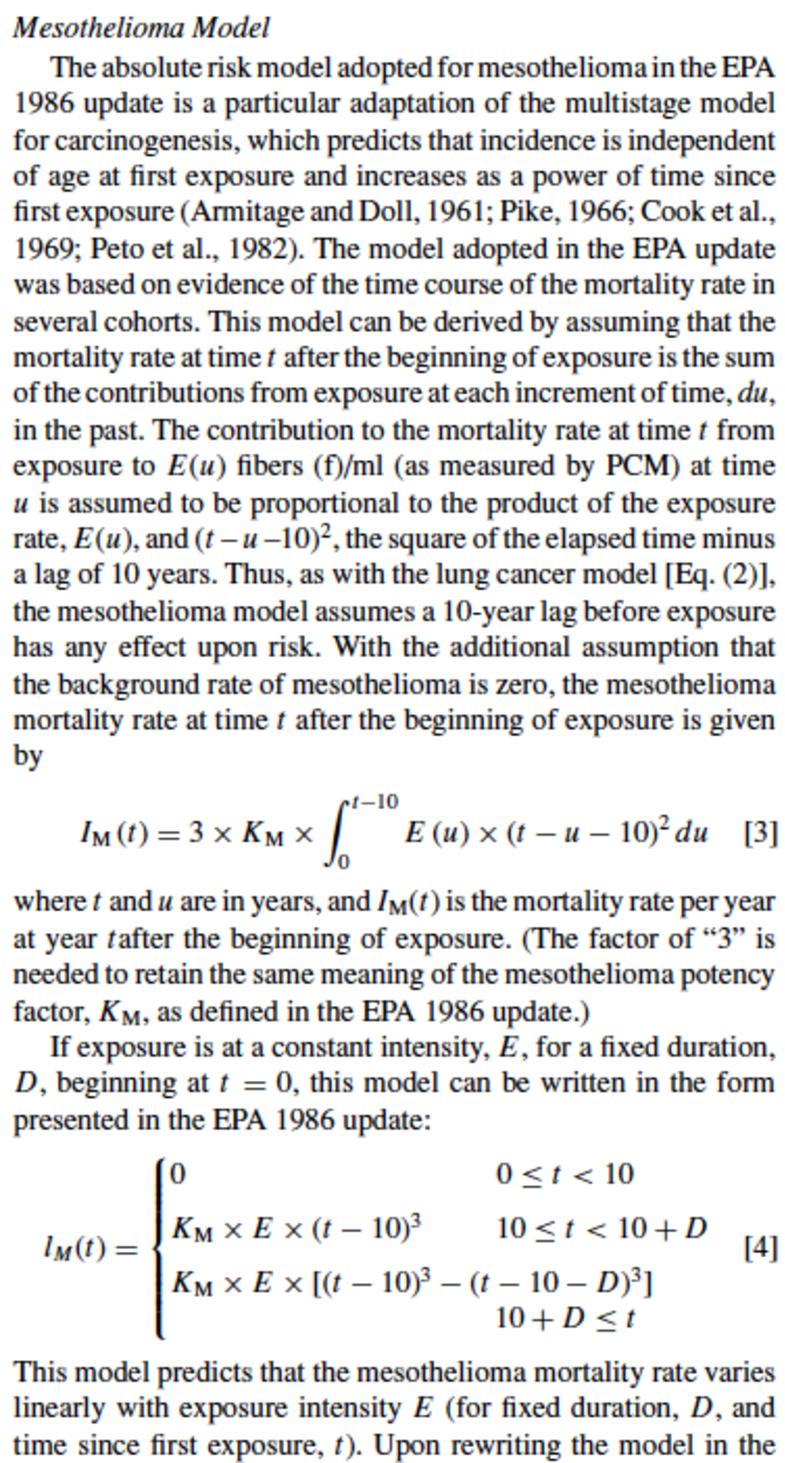
\includegraphics[width=3.5in]{EPA_meso_model}
      \caption{The 1986 EPA mesothelioma model, from Berman and Crump.}
\end{figure}

\FloatBarrier
\section{Previous vesions of the HSE model}

\section{Historic incidence data for model fitting}

\subsection{U.S. data}

Recent (1999-2009) U.S. mesothelioma incidence data come from the USCS (United States Cancer Statistics) system.  This is a collection of registries that covers 98\% of the U.S. population.  Navigating the USCS website poses some challenges.  As of 9/03/13, the full downloadable data (all cancers, not just mesothelioma) live \href{http://www.cdc.gov/cancer/npcr/uscs/download_data.htm}{here}.  You can produce interactive tables of incidence by age and sex \href{http://apps.nccd.cdc.gov/uscs/cancersbyraceandethnicity.aspx}{here}.  These tables are useful for checking computer programs for extractiong mesothelioma data from the full downloads.  Also, if you need a quick download, you can download the interactively-produced age by incidence tables.  You can create and download corresponding U.S. population tables here as well. 

Assembling mesothelioma incidence data for the U.S. is more of a pain than it is for other countries.  For years that precede the establishment of the USCS, the only (approximately) comprehensive national tumor registry is the SEER system.  You may already be familiar with this system, in which case you can skip to the next paragraph.  SEER-9 goes back the furthest.  It contains data from nine tumor registries that reporesent a substantial, but nonrandom, portion of the U.S. population.  Nonetheless, many researchers just apply incidence rates from SEER-9 to U.S. population counts (by sex and age group) to get estimated national incidence counts.  In the micro-world of asbestos disease estimation, there have been papers about "coastal bias".  These articles describe attempts to adjust for the fact that mesothelioma cases come disproportionately from coastal areas, due to shipbuilding exposure.  The SEER-9 data (it is argued) provide a skewed view of the U.S. because they don't adequately represent coastal regions.  I mention this issue just an historical aside -- it doesn't really affect what we're doing.

Additional registries have been added to SEER over time, so as the years advance we start seeing, in addition to the SEER-9 series (which continues to be provided), SEER=11 and SEER=13.

For the U.S., the gold standard is the USCS.  So the analytic challenge in building a complete historic record of U.S. incidence is to impute what USCS would have looked like had it been in existence as long as SEER-9 has.

ARPC and I have both done this kind of imputation, but the methods have been pretty crude.  For initial fits of the HSE model, I suggest that you use UK and Australian meso incidence data.  These data are provided in easily used formats, and tend to be more up-to-date than the U.S. data.  In addition, since most of the development and use of the HSE model has been in these two countries, we can compare our initial fits and predictions to fits and predictions that have been published.  (I'm not looking for identical results -- our data are likely to be of slightly different vintage, and there are a variety of minor tweaks that have been made to the HSE model by different analysts.)

\subsection{OECD data}

Most countries report their data cancer incidence to the OECD in a reasonably timely fashion.  So the OECD data, which are publicly available online, represent a source from which we can get incidence data in a standard format.  If we ever feel like it, once we get the mdel fitting where we like it, we could write an article or build a website in which we report meso forecasts by country.  So work on your shiny and markdown chops. The U.S. reports only the USCS data to the OECD.  It is usually more laggard than other developed counteries about doing this in a timely fashion.

\subsection{Use of mesothelioma incidence data in fitting HSE and releated models}

Incidence data for HSE (and similar) model fitting pose the same challenges as demographic data do for HSE fitting: (1) going from grouped data to "by single year of age", and (2) extending the oldest age interval to single years of age, or to some finer grouping levels.  See the section below on demographic data.  Usually, parallel methods are used for the demographic and incidence data.

Ad hoc methods are often necessary for breaking the oldest age interval into finer categories.  For example, Australian data usually go through age 85+, and UK datq through age 90+.  For most purposes, it would be adequate to more finely bin the Australian date by making use of the ratio (UK 90+ count) / ( UK 85+ count).

Another issue with regard to use of incidence data in our context is that at different times we deal with one or more of three different dates associated with a case of mesothelioma: 

\begin{itemize}
  \item Date of diagnosis (i.e., incidence)
  \item Date of death
  \item Date a claim is filed against a particular trust
\end{itemize}

This issue doesn't matter much for current purposes, as these three dates tend to be within a year or two of each other.  Mesothelioma is almost always fatal within a fairly short period of time, and U.S. attorneys are very efficient at identifying and signing up claims.  (The most expensive search term on Google for buying paid ads is "mesothelioma".)  In some expert analyses, the distinctions across these dates are ignored.

However, it is also reasonable to assume something like a 1-year or a 2-year lag between incidence and filing, particularly forecasting. In forecasting, it might make sense to assume that the decline (aka "runoff") curves for claims lag the national incidence decline curves by a couple of years.

Some other issues in terms of processing data on the claims end are:

\begin{enumerate}
  \item Claims during a bankruptcy proceeding are stayed -- i.e., firms are prohibited from filing them even they would have been filed against the debtor had the debtor not filed for Chapter 11 bankruptcy.  So at the beginning of a trust, there is a catch-up period (usually up to an initial statute of limitations (SOL) date that is typically three years after the initial claims received date) when a lot of the claims would have been filed earlier.  You will see the term "date arising" or "year arising" in some of the claims data that we receive, which translates to "year would have been filed."
  \item Some mesothelioma claims are filed in the tort system against solvent defendants.  If there is a judgment in favor of the plaintiff, usually there is a damage award that is apportioned among the codefendants.  If the plaintiff has settled a claims with one of the codefendants, then that settlement amount may be subrtracted from the total award.  So sometimes a law firm will hold off on filing a claim with any trusts, because then the claim has not been settled with regard to the defendants associated with the trusts, and there is no offset to the tort system award.  Only when the claim is "finished" in the tort system is it filed with the trusts.  This can create a longer gap between diagnosis and filing than the 1-2 years I cited above.
  \item Sometimes there can be a delayed diagnosis.  For example, recently a lot of lung cancer claims were filed because law firms started reviewion x-rays of workers who died of lung cancer, and who had some exposure to asbestos in the workplace.  Many such claims are not filed against asbestos trusts, because the likely cause of the lung cancer is smoking.  However, if there is x-ray evidence of asbestosis in addition to lung cancer, the claim is compensable according to most trust TDPs.  Here again is a situations in which the diagnosis dates in our claims data may not correspond to diagnosis dates that would be counted in public health systems.
\end{enumerate}




In R programs provided in the Rstudio project associated with this note, I have collected some UK and Australia incidence data and converted them into R data frames.  I provide some details below.



\subsection{Australia data}

% The hyperref package is smart enough to sanitize the latex special characters in thge following links.
% However the Rstudio editor for Rnw files is not that smart, so the text coloring will change 
% in the editor window until 

Australia mesothelioma data through 2009 were downloaded from a spreadsheet found \href{http://www.google.com/url?sa=t&rct=j&q=&esrc=s&source=web&cd=2&ved=0CFkQFjAB&url=http%3A%2F%2Fwww.aihw.gov.au%2FWorkArea%2FDownloadAsset.aspx%3Fid%3D60129542445&ei=_gEgUujUAZK7sQS664CoAw&usg=AFQjCNHK5mdE14OBYiRGn2mKJ99QdE5JYw&sig2=TLAj4Y0hCvBI8wTttkKUqg&bvm=bv.51495398,d.cWc}{here}.  Government summaries can be found \href{http://www.google.com/url?sa=t&rct=j&q=&esrc=s&source=web&cd=3&ved=0CF4QFjAC&url=http%3A%2F%2Fwww.safeworkaustralia.gov.au%2Fsites%2FSWA%2Fabout%2FPublications%2FDocuments%2F602%2FMESOTHELIOMA%2520IN%2520AUSTRALIA.doc&ei=ZFMjUsSvD-u3sQTbpoGYAQ&usg=AFQjCNE8hcc3odmiMYv0DkJASn3YuihkmA&sig2=LSGsne4YvK1NCYdQa7HKnA&bvm=bv.51495398,d.cWc}{here}.  These links may change when the data are updated.  I found that googling the terms AIHW, mesotheloma, and data got me to the desired sites.

\begin{figure}[ht]
\vspace{.3in}
\centering
\begin{knitrout}
\definecolor{shadecolor}{rgb}{0.969, 0.969, 0.969}\color{fgcolor}
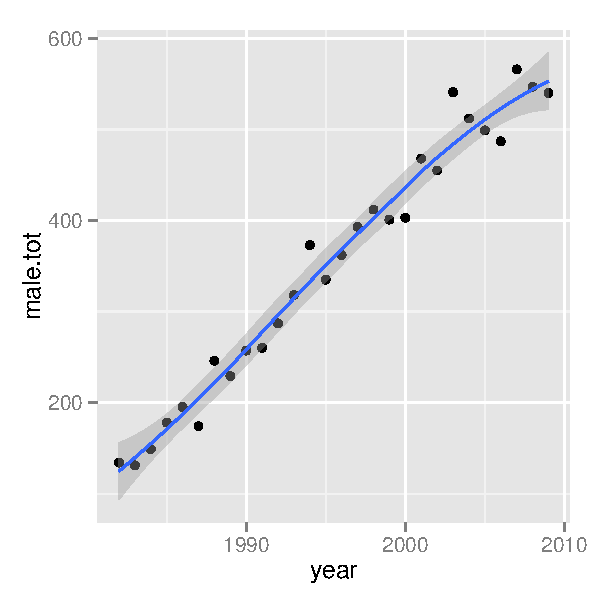
\includegraphics[width=4in,height=4in]{figure/Chunk-aussie-males} 

\end{knitrout}

\caption{ Mesothelioma incidence - Australia males}

\vspace{.3in}
\end{figure}


\FloatBarrier

\subsection{UK data}

UK mesothelioma data through 2010 can were downloaded from a spreadsheet found \href{http://www.hse.gov.uk/statistics/tables/index.htm#lung}{here}.  These UK data reflect date of death, not date of diagnosis.  

\begin{figure}[ht]
\vspace{.3in}
\centering
\begin{knitrout}
\definecolor{shadecolor}{rgb}{0.969, 0.969, 0.969}\color{fgcolor}
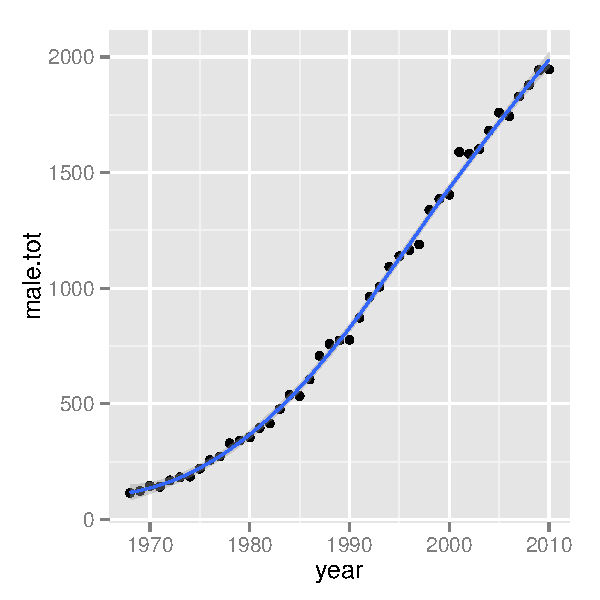
\includegraphics[width=4in,height=4in]{figure/Chunk-uk-males} 

\end{knitrout}

\caption{ Mesothelioma incidence - UK males}

\vspace{.3in}
\end{figure}

\FloatBarrier



\section{Demographic data for model fitting and forecasting}


Population counts are used as an exposure variable in the Poisson regression, and in forecasts made from it.  Historic population counts and death rates can be obtained from the Human Mortality Database.  See the program "Get populations and death rates" in the Rstudio project that accompanies this note.  The program downloads population and death rates for Australia, UK, and US, by gender.  The counts and rates are 1x1 -- age is not grouped, and there counts and rates for each individual year -- but can obviously be grouped if grouping is desired for consistency with meso incidence data.

This R program also uses the demography package to generate Lee-Carter projections of the death rates.  These projected death rates can be used to translate the most recent population counts into future counts, for use in the HSE model projections.  Once we (well, you) have fit a satisfactory HSE model, we should probably do one projection just assuming that the most recent historic death rates will remain constant, and one using the projected death rates that continue to decline.

In my past projections of U.S. mesothelioma incidence using an HSE model, I relied on the historic and projected death rates that the Social Security Administration uses.  See \url{http://www.ssa.gov/oact/NOTES/as120/LifeTables_Body.html}, authored by the wonderfully named Felicitie Bell (Who wouldn't trust a forecast from her?).  I had a number of conversations with her back when I was projecting future tobacco mortality and health care costs for the U.S. DoJ civil rico case against the tobacco companies.

I have all of those SSA rates in R formats from my previous work, both with tobacco and with my HSE modeling.  For now, I suggest we use the Lee-Carter projections for all three of our countries.  We can plug the SSA stuff in later on.  I have read that the SSA uses Lee-Carter projections, although that doesn't really seem to be the case based on Felicitie's description.  I'm not a demographer, so keep that in mind.  I think there are a number of newer methods of death rate projections that do better than Lee Carter by some measures, but Lee-Carter still seems to be the most commonly applied method.

\begin{figure}[ht]
\vspace{.3in}
\centering
\begin{knitrout}
\definecolor{shadecolor}{rgb}{0.969, 0.969, 0.969}\color{fgcolor}
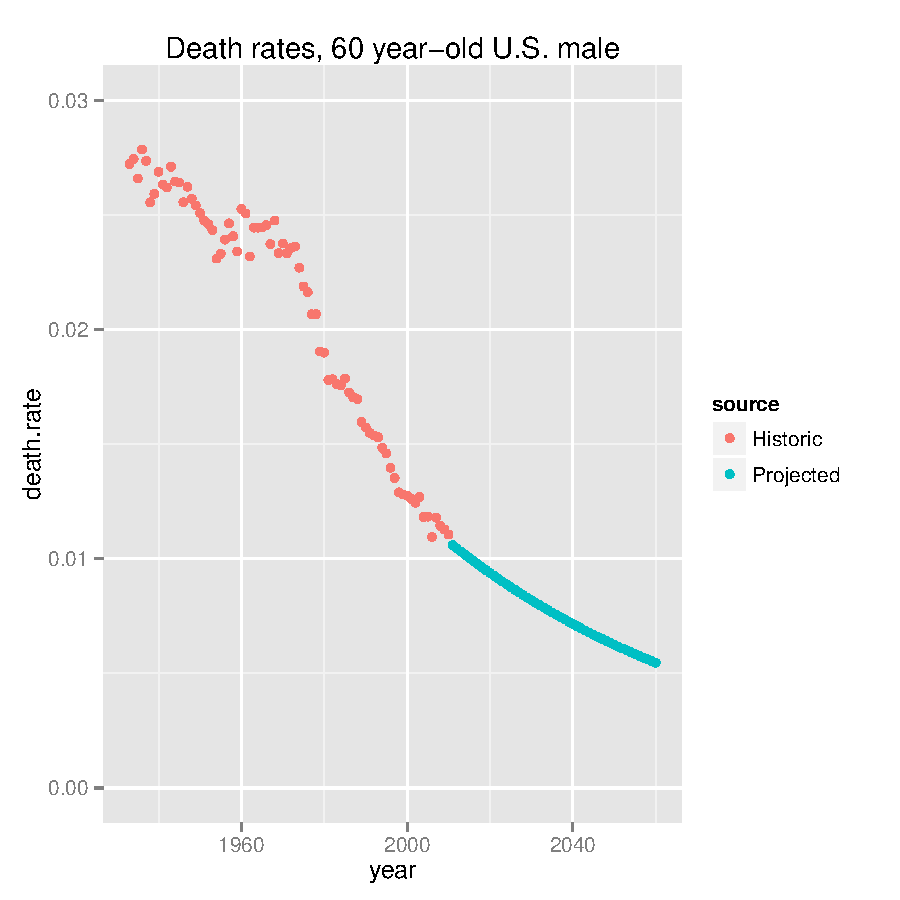
\includegraphics[width=6in,height=6in]{figure/Chunk-us-demographic-example} 

\end{knitrout}

\caption{ U.S. historic and projected death rates by year, 60 year-old men.}
\vspace{.3in}
\end{figure}

Projected mesothelioma cases (and claims) increase if future death rates decrease, because when people live longer they are more likely to contract cancers like mesothelioma.  One issue that nobody but me seems to have thought about in making projections for estimating ultimate trust liabilities is that our exposed workforce may have lower median income than the U.S. as a whole.  (Or maybe not so much -- insulators (for example) don't usually become wealthy, but they were at least employed, frequently in well-paying union jobs.)  I suggest that we ignore this issue for now.  Down the line, we might want to think about it.  I provide some references in the accompanying material.\footnote{ Donkin (2002), Singh (2006), Waldron (2007)} In my previous HSE forecast, I adjusted death rates upwards using the Donkin articles.

\FloatBarrier


\section{Previous fits of the HSE model}

\subsection{ Initial HSE model(s)}
The HSE model was first described in an HSE working paper\footnote{HSE (2003)}, which subsequently became an article in BJM.\footnote{Hodgson (2005)}.  I relied on these articles for my own HSE fit.  The analysts used a lot of degrees of freedom to describe exposure as a function of age and of calendar year.  They used some kind of ad hoc methods that seem a bit antiquated, like what one would expect from some clever statisticians with roots in Bletchely Park who were reared to think of computer runs as an unseemly expense, to be minimized whenever possible.  

Nonetheless, I followed their model pretty faithfully.  I fit it using optim(), with an option that allowed me to put bounds on the estimates for each parameter.  These were needed because, with all the degrees of freedom, the marginal likelihood for some parameters was dead flat, and iterations would wander off into never-never land.  Fitting was also very slow, because the optimizer called my likelihood function many times, and each time there were a lot of inefficient summations performed to construct the likelihood with current parameter values.  I figured out how to do the summations via matrix multiplication, which should be much faster, but never had time to return to work on this project.  Some charts of goodness of fit of my application to U.S. data occur in the latter part of a slide presentation in the accompanying material.\footnote{Wyant (2011)}  (The initial slides in this document relate to a revision of the Peto model -- see the previous section on different meso forecasting methods.)

Several other HSW tweaking issues are:

\begin{enumerate}
  \item The model does not yet include an estimate of background risk.
  \item The model at this point is only for males.
  \item The age range is somewhat narrow.
  \item A lot of emphasis is put on the "diagnostic trend" term -- accounting for possible missed cases in earlier years.  This element is given less emphasis -- or none at all -- in subsequent modeling efforts.  In Hogsdon (2005), the authors note that presence or absence of this term has essentially no impact on forecasts.
  \item The original model in the HSE working paper assumed a long clearance half life of asbestos fibers from the lung.  Effectively, "no clearance" was assumed.  The assumption of nonclearance is not always made in subsequent models.  In the followup Hogsdon (2005) journal article, the authors fit both a clearance and a nonclearance model.  The two models gave very similar fits and forecasts.\footnote{Two of the model
parameters, k (the power of time defining the increase in risk
after exposure) and H (the half-life for clearance of asbestos from
the lung), are closely correlated and cannot be independently
estimated. The effect of reducing the half-life is to increase the
best-fit value of k, but the fit of the model is affected only slightly.
Since fitting the model with both H and k is unstable, we used two
versions of the model, one with (effectively) no clearance
(H¼1000 years) and the other with a clearance half-life of 15
years – a value suggested from the modelling of mortality of the
Wittenoom workforce (Berry, 1991).  Page 587.} 
  
The power of time since first exposure, \emph{k}, is hard to estimate independently of the clearance half life -- they are negatively correlated.  The nonclearance model gives \emph{k} within the 2-3 range, as was expected, and also yielded an exposure index over time that more closely matched the pattern of asbestos imports over time.  For these reasons, the authors expressed a (mild) preference for the nonclearance model. 
  \item The model fits the power of time since first exposure, and gets a vale between 2 and 3 -- consistent with what one wouuld expect from the EPA 1986 models discussed above.  Subsequent fits of the the HSE model by these and other analysts sometimes just treat the power as fixed, and some (notably ARPC) calculate a fitted value that is less than 2 (something like 1.8, if I recall).
  \item The predicted peak number of mesothelioma deaths in the UK is about 2,100.
\end{enumerate}

\subsection{ Bayesian refitting of the original HSE model(s) with MCMC }

HSE analysts refit the HSE model using a Bayesian approach.\footnote{ HSE RR728 (2009), the HSE working paper, and Tan and Warren (2010), the subsequent journal article.}  As usual, there were tweaks to the model.  Many of the tweaks were just minor fiddling with the binning of the indices of exposure over time, and exposure by age.  One substantive addition was that of a background exposure rate parameter.  Background exposure was assumed to be related to age.\footnote{The background rate is represented by the number of cases per million in the male population. The age distribution of
the background cases in each year is assumed to be (A-L)\textsuperscript{k}. Page 431.} 

The clearance half-life was set at 1,000,000.  This is really a nonclearance model! And, of course, the Bayesian framework allowed for the calculation of prediction intervals.  Basically, though, the fit and the projections from the model are by and large similar to what was produced with earlier classical optimization routines.  Note that we have several years more incidence data with which to fit our HSE model than was used in any of the model fits I have so far described.

\subsection{Adoption of the HSE model(s) by actuarial societies and public health analysts}

Actuarial societies in the UK\footnote{Gravelsons (2010).} and Australia\footnote{I couldn't find the reference right away, but I think it's by Lowe.} did public, systematic reviews of available mesothelioma forecasting models and selected the HSE model as the best.  The UK insurers face about \$18 billion in estimated liability for such claims.  Some public health analysts in Australia started using HSE models as well.\footnote{Clements (2007a) and Clements (2007b)}

\subsection{Initial use of the HSE model(s) in the U.S. asbestos trust world}

I fit a version of the HSE model to U.S. data in 2010, as I have mentioned in a couple of places.\footnote{ Wyant (2011), which also discusses revision of the Peto model.}  When ARPC saw my stuff, they decided to both revise their Peto model, and do their own fit of the HSE model.\footnote{ ARPC (2011a); ARPC (2011b).}  I consulted with them on both.  ARPC now uses their mode, but they do a simple model averaging of four models.  The HSE model gives the highest forecasts, but because they use the median of their four forecasts, the fact that the HSE models gives substantially higher values than the other three is effectively ignored.

Both my revised Peto and my HSE models seem to yield higher forecasts than ARPC's.  I don't know why.  I would like to revisit this in detail with them at some point, but I want to have carefully gotten all my ducks in a row -- with your help -- before doing so.  One thing about their HSE fit -- they get a \emph(k) value of 1.86 or thereabouts, outside the ideal range of between two and three.

I would also like to launch a campaign with them to put more weight on the HSW result.  One argument is, as I alluded to earlier, is that Stallard and Manton have revised their forecasting model and are now getting forecasts more like our HSE forecasts -- about 30\% higher than the old Nicholson model.

\subsection{More recent HSE models -- two-stage clonal and "imports-based"}

Recently, HSE analysts published results of additional model fits.\footnote{HSE RR876 (2011).}  The working paper has the regrettable title "... revised and two-stage clonal models."  A better summary of what they did is:

\begin{enumerate}
  \item Fit one alternative "imports-based" HSE model in which historic annual imports of asbestos in the UK are used as an independent variable,
  \item Fit a "two-stage clonal" HSE model, an attempt to reflect some recent mathematical models of tumor development,
  \item Fit the "old" HSE model to get a model for women, albeit with usual tweaks to deal with the new data, achieve convergence of numerical methods, etc. -- hence the quotes around "old",
  \item Basically concluded that the "old" HSE model is still the best model.
\end{enumerate}

The tone and style of this report smacks (to me) of either (1) we have all this machinery, let's get a quick publication by fitting a couple of alternative models, or (2) somebody higher than us in the chain of command keeps asking about these other models -- let's just fit 'em to get them off our backs so we can get back to doing something useful.  Unfortunately, the authors of this report did not overtly say that the "old" HSW model is still the model of choice."  This caused someone (after I had given a presentation on our version of the HSE model for the U.S.) to circulate and email to audience members saying that "the HSE has discarded the model that Tim is using."

In fact, what them authors said was:

\begin{enumerate}
  \item The estimated of 2,100 mesothelioma cases at the peak is still our best estimate [this is the estimate from the old HSE model],
  \item The upper bound on future mesothelioma cases is the upper bound calculated for the old HSE model, and
  \item The way we will fit the model for women is the old HSE model (with the usual tweaks and upgrades).
\end{enumerate}

This all says to me that they still think the old HSW model is the best practice -- they just don't say so in a simple declarative sentence.

The notion of an "imports-based" model makes some intuitive sense.  Using imports (or mining output, but in the cases of the UK and the U.S. import almost all the asbestos is imported) should add information.  In the UK, it doesn't matter much.  The index of asbestos exposure over time produced by fitting the HSE model mirrors pretty closely the import records.  (In fact, some of the earlier HSE papers use "closeness to imports" as a guide in choosing between a couple of model tweaks.)

In Australia, the actuarial society (or somebody like that) compared different forecasting models, including the imports-based model (in Australia, probably the mining-based model) -- which they called the "latency model" (who knows why) -- and concluded that the imports-based model did not fit well, and that the HSE model was superior.

My fit of the HSE model yielded an index of exposure over time that does not match the record of U.S. imports.  I have no idea why.  Poor imports data (e.g., how much was then re-exported?).  Some mistake that I made?  Change in the mix of manufacturing and construction processes that use asbesto, with resulting changes in intensity of exposure?  Change in the type of processes?  Change in job safety standards?  (Nobody seems to believe the latter.)  Who knows.  In any event, once you have fit a new HSE model for the U.S., a subsequent step will be to fit an imports-bassed model.  The U.S. imports data are in the accompanying materials.\footnote{USGS (1997)}

I don't know anything about the two-stage clonal model, but we should look at fitting that one once we have gotten more important things out of the way.


\section{Our HSE modelling plan}

The word "template" is too strong, but I would like to use something like the model fit by CLements\footnote{Clements 2007b} as a starting point.  See Figure 5. 

\begin{figure}[h!]
  \centering
    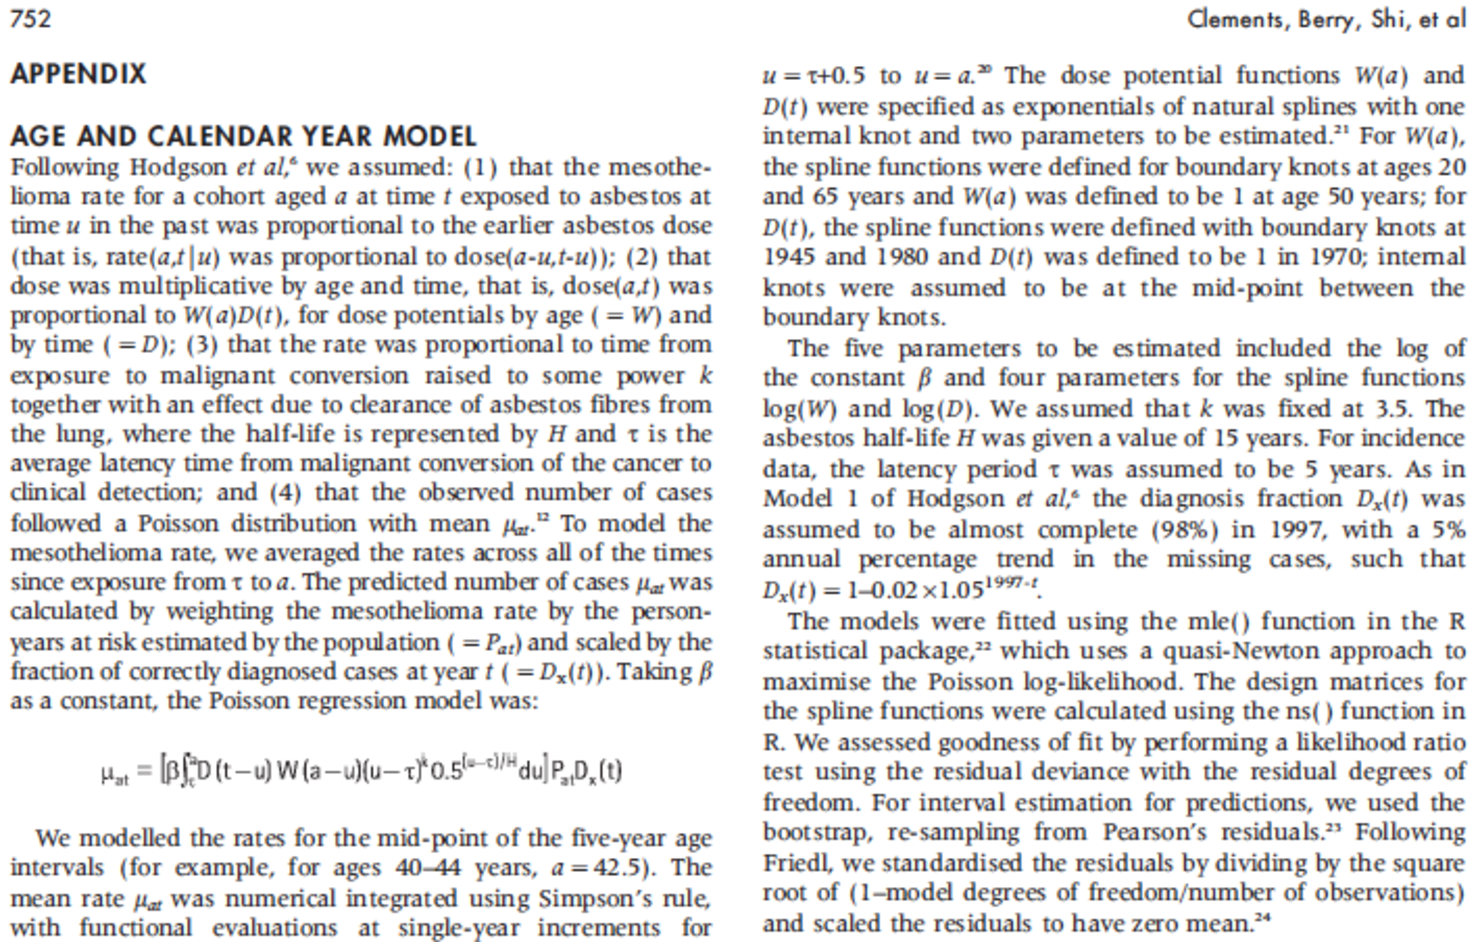
\includegraphics[width=6in]{Clements_technical_appendix}
      \caption{Clements 2000b technical appendix.  Possible starting point for our HSE fit.}
\end{figure}

Here are my thoughts about working off of this model:

\begin{enumerate}
  \item I don't like the HSE's baseline HSE model (and the similar one that I originally fit using optim()) because it uses too many degrees of freedom and too ad hac an approach to building indices of exposure over time and exposure as a function of age.  I thought splines would be a better way to go -- as did Clements.  However, I'm not totally sold on his splines.  I do think some assymetry in the indices is good to incorporate, which to me means perhaps three degrees for freedom for each of the two splines, not two.  I haven't quite followed the significance of his knot placement.  I think I understand roughly how he's forcing the indices to have fixed values at certain points, but my level of understanding is probably lower than I think.  Anyway, we're into your territory now, so I leave you to deal with this issue, and (I hope) educate me a bit.
  \item I don't know about using numeric integration, rather than discrete summing.  Discrete summing can be slow, as I found out, but could presumably be speeded up by matrix multiplication or other cleverness.  Plus, fits will go faster simply due to usine fewer and better-defined independent variables.  Anyway, I again turn to you.  Maybe numeric integration is the bee's knees.
  \item As other articles I have cited would indicate, halflife and the k exponent are negatively correlated, and models that try to fit both of them are unstable.  I don't know why Clements chose to make both of them fixed, and at extreme values.  (They're not extreme in a way -- due to the negative correlation you can get the same fit making the exponent big and the halflife small as you get with more moderate values.)  Given the discussions in the other articles, I would tend to fit \emph{k} and ignore half-life -- or fix halflife at 1,000,000 years as one paper did.  For one thing, there is some biological validation of our fit if the estimated \emph{k} is between 2 and 3, as it was in my fit of the HSE model.
  \item I think beta in the Clements model is basically the background rate.  I would like to fit a background rate.  As discussed above, assuming that the background rate increases with age makes sense -- we might add that.  This is not a big issue in a way, as background rates are small.  But it again lends some biologic validation to our model if we fit a background rate and it is indeed small.
  \item Clements uses stats4::mle(), rather than optim().  Of course, mle() is just a wrapper for optim().  I have not used mle(), but it has seemed to me a good thing to consider where (as here) one is optimizing a likelihoodl.  It would seem to clarify how exactly we are using a poisson regression (not clear at all in the early HSE papers), and I think could yield some initial error bounds by numericalluy inverting the second derivative matrix. There is also now bbmle::mle2() to consider.  Anyway, I leave all this in your capable hands, hoping again for some education down the line that is simple enought for me to absorb.
  \item In U.S. meso incidence data, I have noticed a flattening in the incidence rates somewhere above age 80.  This may reflect underdiagnosis.  If an oldster in a nursing home with pneumonia dies, I don't think anybody will be requesting an autopsy to see if there is something else going on in the lung region.  However, "flattening" has been an issue from time to time in the meso modeling literature.  Some analysts find it hard to believe that risk can go up indefinitely as a power of two or three.  But in any event, I have found it useful to build in a "flattening age" like at 85 in my modeling. You might consider doing the same, at least as a check.
  \item I don't know about fitting to midpoints of age ranges, as Clements does.  Certainly it should make initial fitting routines run a little faster.  In the past, I have converted to single-year-of-age by applying splines to cumulative incidence by age in each calendar year.  It would certainly seem necessary to do something like this in the forecasts, where we need annual forecasts and it is hard to calculate how many people move from one age group to the next in a year without -- you know -- actually calculating what happens at the single year of age level.  But I again leave this kind of pondering to you. 
  \item I think (I think you would have done this anyway) we should get a standard numerical fit before moving on to Rjags.  I also think we should start by fitting to UK and/or Aussie data, as these data are tidy, and the we can also check our fit against the several fits in the literature.
  \item You would do this anyway, but just so I have a reminder here for myself -- the modeling programs should generate the kinds of diagnostic fit plots that appear in my and ARPC's presentations\footnote{ARPC 2011a, Wyant 2011}, including plots of the indices overlaid by import data, and also some measures of goodness of fit like log-likelihood, AIC, etc.  And we need some error bounds on forecasts and on parameters such as \emph{k}.
  \item Next up in rough priority after doing a new "standard" U.S. male model is to:
  \begin{enumerate}
  \item Compare with my and ARPC's HSE fits,
  \item Do some forecasts for individual trusts -- as I say, this has been done by outputting historic and projected U.S. national counts by birth cohort group, identifying a stable claimiing period in the trust history, calculating trust to U.S. ratios by birth cohort, and then applying these ratios to the projected U.S. counts from the HSE model.;
  \item Do a female model,
  \item Do a combined forecast of male plus female,
  \item Fit some kind of imports-based model,
  \item Take a look at the two-stage clonal model, and
  \item Look at an Rjags fit.
\end{enumerate}

\end{enumerate}





\end{document}
